\documentclass[dvipdfmx]{standalone}
\usepackage{tikz}
\usetikzlibrary{positioning}
\usetikzlibrary{patterns}
\usetikzlibrary{intersections, calc}
\usetikzlibrary{datavisualization}
\usepackage{pxpgfmark}


\begin{document}
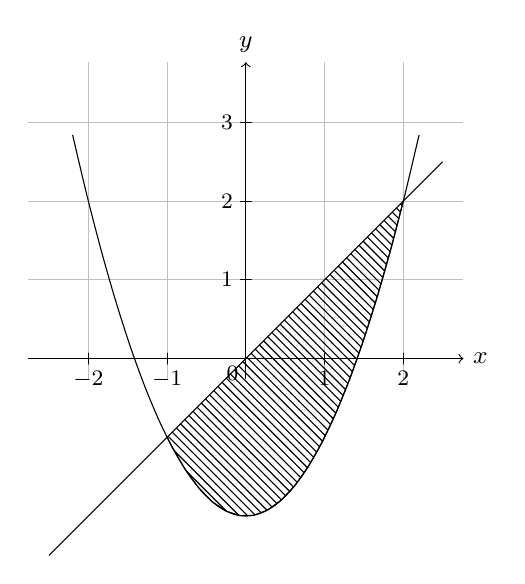
\begin{tikzpicture}
  \datavisualization[
  school book axes,
  x axis = {label = {$x$}},
  y axis = {label = {$y$}},
  all axes = grid
  ]
  data{
  x,y
  -2.5, 2.5
  2.5, 3.5
  };
  %
  \begin{scope}
    \draw[domain=-2.5:2.5] plot(\x, \x);
    \draw[domain=-2.2:2.2, smooth] plot(\x, {\x*\x-2});
  \end{scope}
  %
  \begin{scope}
    \clip(-2.5, -2.5) |- (0, -2.5) -| (2.5, 2.5) --cycle;
    \clip[draw, domain=-2:2.2] plot(\x, {\x * \x -2});
    \draw [pattern=north west lines](-2.5, -2.5) rectangle(2.5, 3.5);
  \end{scope}
\end{tikzpicture}

\end{document}
